%%%%%%%%%%%%%%%%%%%%%%%%%%%%%%%%%%%%%%%%%%%%%%%%%%%%%%%%%%%%%%%%%%%%%%%%
\chapter{AC circuits}

\section{AC sources}
AC sources produce voltages or currents that change with time. In a sense all sources change with time because no sources have been steady for longer than the age of the universe. But some sources are steady enough that we treat them as DC sources.\\
\\
The frequency of an electrical source represents the number of cycles per second. One cycle per one second is called a Hz (Hertz). The frequency of a wall socket is 60 Hz, or 60 cycles per second. A 9V battery might undergo 1 cycle in 5 years for a frequency of $\frac{1}{5*365*24*60*60}$ Hz. \\

\begin{alevel}
What would be the frequency (in Hz) of a current source that turned on and off 5 times per minute?
\end{alevel}

\begin{figure}[H]
\begin{center}
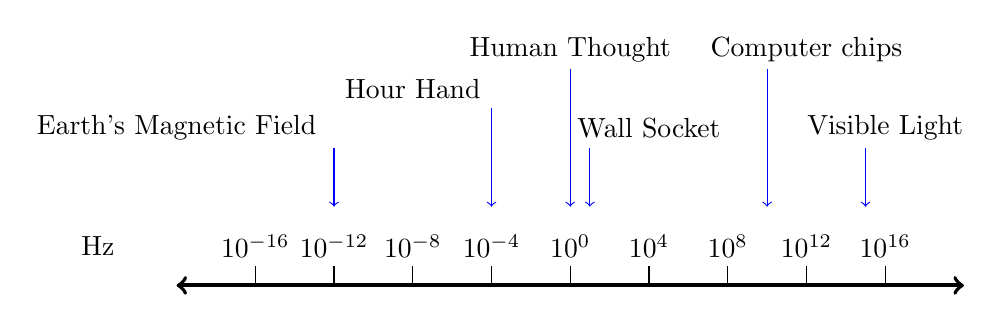
\begin{tikzpicture}
\draw (1,0)--(1,.25);\draw (2,0)--(2,.25);
\draw (3,0)--(3,.25);\draw (4,0)--(4,.25);
\draw (5,0)--(5,.25);\draw (6,0)--(6,.25);
\draw (7,0)--(7,.25);\draw (8,0)--(8,.25);
\draw (9,0)--(9,.25);
\draw [line width=0.5mm] [<-](0,0)--(2,0);
\draw [line width=0.5mm] [->](2,0)--(10,0);
%\filldraw (0,2) circle[radius=1 mm];
\draw node at (1,.5) {$10^{-16}$};\draw node at (2,.5) {$10^{-12}$};
\draw node at (3,.5) {$10^{-8}$};\draw node at (4,.5) {$10^{-4}$};
\draw node at (5,.5) {$10^{0}$};\draw node at (6,.5) {$10^{4}$};
\draw node at (7,.5) {$10^{8}$};\draw node at (8,.5) {$10^{12}$};
\draw node at (9,.5) {$10^{16}$};
\draw node at (-1,.5) {Hz};
\draw node at (9,2) {Visible Light}; \draw [draw=blue] [->] (8.75,1.75)--(8.75,1);
\draw node at (8,3) {Computer chips}; \draw [draw=blue] [->] (7.5,2.75)--(7.5,1);
\draw node at (5,3) {Human Thought}; \draw [draw=blue] [->] (5,2.75)--(5,1);
\draw node at (3,2.5) {Hour Hand}; \draw [draw=blue] [->] (4,2.25)--(4,1);
\draw node at (6,2) {Wall Socket}; \draw [draw=blue] [->] (5.25,1.75)--(5.25,1);
\draw node at (0,2) {Earth's Magnetic Field}; \draw [draw=blue] [->] (2,1.75)--(2,1);
\end{tikzpicture}
\caption{Comparisons of various frequencies. The horizontal axis uses a log axis: each tic-mark goes up or down by a factor of 10.}
\end{center}
\end{figure}

\begin{blevel}
Determine, exactly, frequency (in Hz) of the hour hand on a clock.
\end{blevel}

Consider an AC source, like $V=3sin(2t)$. The average voltage is zero, because the average output of the sin function is zero. The amplitude is 3V and it has an angular frequency of $2 \frac{radians}{s}$. This voltage source will repeat whenever the input to the sin function increases by $2\pi$ radians. This will occur when:\par

\begin{align*}
2\pi=2t\\
t_{repeat}=T=\pi(s)
\end{align*}

The time to repeat is called the period and its symbol is T. Period is $\frac{time}{cycle}$. Frequency is $\frac{cycles}{time}$. There is an inverse relationship between period and frequency, $T = \frac{1}{f}$.

\begin{blevel}
Suppose a steering wheel vibrates with a period of 0.125 seconds. How many cycles does the wheel undergo each second? 
\end{blevel}

\begin{alevel}
How many radians are in one cycle?
\end{alevel}

\begin{blevel}
A piece of equipment produces a sinusoidal voltage at a frequency f of 30 Hz. What is the period? What is its angular frequency, $\omega$?
\end{blevel}

The blue line of figure~\ref{F:8PHASE} graphs the voltage across this AC source as a function of time.

\begin{figure}[H]
\begin{center}
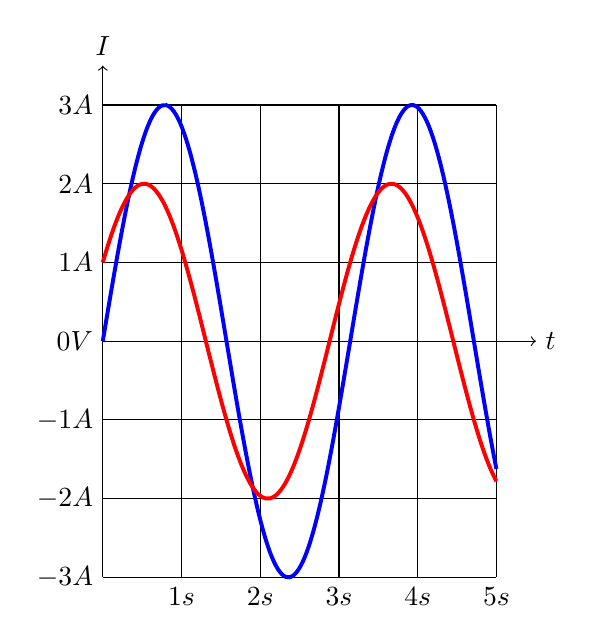
\begin{tikzpicture}
\draw[->] (0,0)--(5.5,0) node[right] {$t$};
\draw[->] (0,-3)--(0,3.5) node[above] {$I$};
\draw (0,0)node[left, line width=0.5] {$0 V$} --(5,0);
\draw (0,-3)node[left] {$-3 A$} --(5,-3);
\draw (0,-2)node[left] {$-2 A$} --(5,-2);
\draw (0,-1)node[left] {$-1 A$} --(5,-1);
\draw (0,1)node[left] {$1 A$} --(5,1);
\draw (0,2)node[left] {$2 A$}--(5,2) ;
\draw (0,3)node[left] {$3 A$}--(5,3) ;
\draw (1,-3)node[below] {$1 s$}--(1,3) ;
\draw (2,-3)node[below] {$2 s$}--(2,3) ;
\draw (3,-3)node[below] {$3 s$}--(3,3) ;
\draw (4,-3)node[below] {$4 s$}--(4,3) ;
\draw (5,-3)node[below] {$5 s$}--(5,3) ;
\draw [draw=blue, line width=.5 mm,smooth, samples=100,domain=0:5,xscale=1,yscale=1] plot(\x,{3*sin(57.29*2*\x)});
\draw [draw=red, line width=.5 mm,smooth, samples=100,domain=0:5,xscale=1,yscale=1] plot(\x,{2*sin(57.29*2*\x+30)});
%\draw [draw=blue, line width=.25 mm, dashed] (0,2.5)--(5,2.5);
\end{tikzpicture}
\caption{Current as a function of time}
\label{F:8PHASE}
\end{center}
\end{figure}

Compare that with this voltage source:$V_2=2sin(2t+30^o)$, also shown in red on the graph. This $30^o$ value is called the phase shift because it is shifted by $30^o$, or $\frac{1}{12}$th of a cycle, or a couple tenths of a second.

\begin{alevel}
If the phase difference between the blue and red signals is $30^o$, which source leads (comes first in time)?
\end{alevel}

\begin{alevel}
Write down any two voltage signals that are 45 degrees out of phase with each other.
\end{alevel}

\begin{alevel}
What is the period of the red signal? What is its amplitude?
\end{alevel}

\begin{blevel}
Fill in the Table~\ref{T:AC1}.
\end{blevel}

\begin{table}[H]
\begin{center}
\begin{tabular}{|c|c|c|c|c|c|} \hline
source&amplitude	&period	&angular frequency	&frequency &units of bolded value \\ \hline
V=\textbf{3}cos(5t)&		&&&& \\ \hline
I=5cos(\textbf{3}t)&		&&&& \\ \hline
I=5cos(3(t+\textbf{1.2}))&		&&&& \\ \hline
I=5cos(3t+\textbf{1.2})&		&&&& \\ \hline
\end{tabular}
\caption{Practice with AC source terminology}
\label{T:AC1}
\end{center}
\end{table}


%%%%%%%%%%%%%%%%%%%%%%%%%%%%%%%%%%%%%%%%%%%%%%%%%%%%%%%%%%%%%%%%%%%%%%%%%%%%%%%%%%%

\subsection{RMS Values}
Consider trying to measure a 60Hz AC source with a meter. The meter would need to switch from positive to negative values 60 times per second.  The meter will probably have trouble keeping up \footnote{And even if it could, the human eye couldn't see it.} and will settle on the average value.

\begin{alevel}
What is the average value of any sin(..) function over a full period? How about over two full periods?
\end{alevel}

One could use an oscilloscope, but often another method is used to capture the \emph{size} of an AC signal with one number.  You might consider using the maximum or peak value. That would work well if if we knew the AC signal were sinusoidal.\footnote{For sinusoidal voltages, the maximum would be the magnitude.} However, it won't work well for other periodic sources, like the ones shown in Figure~\ref{F:8RMS}.

\par
\begin{figure}[H]
\begin{center}
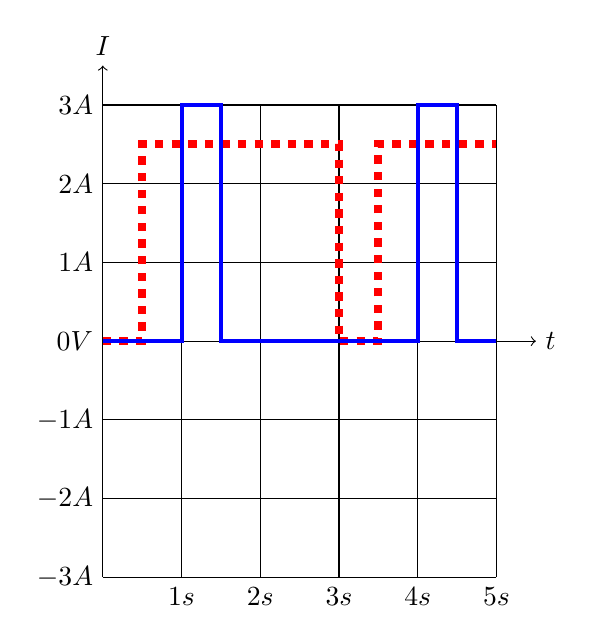
\begin{tikzpicture}
\draw[->] (0,0)--(5.5,0) node[right] {$t$};
\draw[->] (0,-3)--(0,3.5) node[above] {$I$};
\draw (0,0)node[left, line width=0.5] {$0 V$} --(5,0);
\draw (0,-3)node[left] {$-3 A$} --(5,-3);
\draw (0,-2)node[left] {$-2 A$} --(5,-2);
\draw (0,-1)node[left] {$-1 A$} --(5,-1);
\draw (0,1)node[left] {$1 A$} --(5,1);
\draw (0,2)node[left] {$2 A$}--(5,2) ;
\draw (0,3)node[left] {$3 A$}--(5,3) ;
\draw (1,-3)node[below] {$1 s$}--(1,3) ;
\draw (2,-3)node[below] {$2 s$}--(2,3) ;
\draw (3,-3)node[below] {$3 s$}--(3,3) ;
\draw (4,-3)node[below] {$4 s$}--(4,3) ;
\draw (5,-3)node[below] {$5 s$}--(5,3) ;
\draw [dashed, draw=red, line width=1 mm] (0,0)--(0.5,0)--(.5,2.5)--(3,2.5)--(3,0)--(3.5,0)--(3.5,2.5)--(5,2.5);
\draw [draw=blue, line width=.5 mm] (0,0)--(1,0)--(1,3)--(1.5,3)--(1.5,0)--(4,0)--(4,3)--(4.5,3)--(4.5,0)--(5,0);
%\draw [draw=blue, line width=.5 mm,smooth, samples=100,domain=0:5,xscale=1,yscale=1] plot(\x,{3*sin(57.29*2*\x)});
\end{tikzpicture}
\caption{V(t). The red signal is thicker and dashed. The blue signal is taller, thinner and solid. The signals both repeat every 3s.}
\label{F:8RMS}
\end{center}
\end{figure}

\begin{blevel}
What is the frequency of the signal shown in Figure~\ref{F:8RMS}?
\end{blevel}

The peak value would not let us differentiate between the blue and the red signals. To capture the imapcts of each of these signals with one number, we'll introduce a measure called the rms value. rms stands for root of the mean of the square.\\
\\
To determine the rms value of the red signal, we'll divide the period into six, half-second intervals. The red signal takes on the values: \{0,2.5,2.5.2.5,2.5,2.5\}. To get the rms value, we square these values, then take the mean (average) then take the square root. \\

\begin{align*}
0 \hspace{.5cm}2.5 \hspace{.5cm} 2.5 \hspace{.5cm} 2.5 \hspace{.5cm} 2.5 \hspace{.5cm} 2.5\\
0 \hspace{.5cm}6.25 \hspace{.5cm}6.25 \hspace{.5cm}6.25\hspace{.5cm}6.25 \hspace{.5cm}6.25&&\text{After squaring}\\
5.208=\frac{0+6.26+6.25+6.25+6.25+6.25}{6}&&\text{Find the mean}\\
rms=2.28&&\text{After taking root}\\
\end{align*}

\begin{blevel}
What is the rms value of the BLUE signal in Figure~\ref{F:8RMS}?
\end{blevel}

\begin{alevel}
Determine the rms value of a signal that changes from 2 to 0 to 9 Volts, and then repeats, spending equal time at each level.
\end{alevel}

\begin{blevel}
Find an estimate for the rms value of $V = Asin(t)$ by using 8 evenly spaced samples.
\end{blevel}

\begin{dlevel}
Show that the rms value of $V = Asin(t)$ is $\frac{A}{\sqrt{2}}$ by using an infinite number of evenly spaced samples.
\end{dlevel}

\par
People sometimes employ the rms value to indicate surface roughness. Suppose an engineer measures the thickness of a plate at several places to be: \{2,2.01,1.98,2.03,2.01,2.01.1.99,2\}mm. The average thickness is 2.00 mm. The deviations from the average are: \{0,0.01,-0.02,0.03,0.01,-0.01,0\}. The rms value of the deviations provides a sense of how uniform the plate is\footnote{The average of these deviations would be useless, because it would always be zero.}. The rms value would be:

\begin{blevel}
For the thickness measurements on the plate, show that the rms value of the deviation from the average is 0.0151 mm.
\end{blevel}

%%%%%%%%%%%%%%%%%%%%%%%%%%%%%%%%%%%%%%%%%%%%%%%%%%%%%%%%%%%
\subsection{The Wall Outlet}
A wall socket produces an rms value of about 120V at a frequency of 60 Hz. 

\begin{blevel}
What is the peak value of the wall outlet voltage? What is the period of the wall outlet's voltage?
\end{blevel}

%%%%%%%%%%%%%%%%%%%%%%%%%%%%%%%%%%%%%%%%%%%%%%%%%%%%%%%%%%%%%%%%%%%

\subsection{Adding out of phase AC sources}
In this section, we'll see a method to add some AC sources together. Consider two AC voltage sources connected in series.

\begin{figure}[H]
\begin{center}
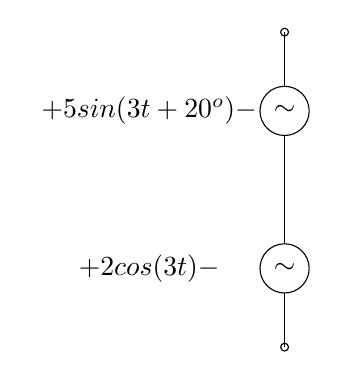
\begin{tikzpicture}
\draw (0,0)--(0,1)node[circle, draw=black,fill=white]{$\sim$}
--(0,3)node[circle, draw=black,fill=white]{$\sim$}--(0,4);
\draw node at (-1.75,1) {$\begin{matrix}+\\2cos(3 t)\\-\end{matrix}$};
\draw node at (-1.75,3) {$\begin{matrix}+\\5sin(3 t+20^o)\\-\end{matrix}$};
\draw (0,0) circle[draw=black,radius=.5 mm];
\draw (0,4) circle[draw=black,radius=.5 mm];
\end{tikzpicture}
\caption{Two AC sources in series}
\end{center}
\end{figure}

The total voltage would be thier sum, but a little simplication can be done with the help of some Euler's equation and leveraging our earlier work with complex numbers.\\
\\
Useful results from chapter 7:
\begin{align}
sin(x)=\frac{e^{ix}-e^{-ix}}{2i} \label{E:8SIN}
\end{align}

\begin{align*}
V_T&=2cos(3 t)+5sin(3 t+20^o)\\
V_T&=2sin(3 t+90^o)+5sin(3 t+20^o)\\
V_T&=2(\frac{e^{3it+90^0}}{2}-\frac{e^{-(3it+90^0)}}{2})
		+5(\frac{e^{3it+20^0}}{2}-\frac{e^{-(3it+20^0)}}{2})&\text{From Equation~\eqref{E:8SIN}}\\
V_T&=\frac{1}{2}(2e^{3it}e^{i90^0}-2e^{-3it}e^{-i90^0}
		+5e^{3it}e^{i20^0}-5e^{-3it}e^{-i20^0}))\\
V_T&=\frac{1}{2}(2e^{3it}e^{i90^0}+5e^{3it}e^{i20^0}-2e^{-3it}e^{-i90^0}-5e^{-3it}e^{-i20^0}))
	&\text{Use $e^{i90^o}=i$, $e^{i20^o}=0.94+i0.34$}\\
V_T&=\frac{1}{2}(e^{3it}(2i+(4.69+1.71i))-e^{-3it}(-2i+(4.698-1.71i))\\
V_T&=\frac{1}{2}(e^{3it}(4.69+3.71i)-e^{-3it}(4.698-3.71i))\\
V_T&=\frac{1}{2}(e^{3it}5.99e^{i38.3^o}-e^{-3it}5.99e^{-i38.3^o})\\
V_T&=5.99\frac{e^{i(3t+38.3^o)}-e^{-i(3t+38.3^o)}}{2}\\
V_T&=5.99sin(3t+38.3^0) &\text{Combined Source}
\end{align*}

It can seem a little intimidating, but we'll using this kind of work with complex numbers and you might as well get comfortable now.

\begin{clevel}
Use the same procedure (show steps) to combine these two voltage sources in series: $V_1=5cos(10t)$ and $V_2=7sin(10t+55^0)$.
\end{clevel}

%%%%%%%%%%%%%%%%%%%%%%%%%%%%%%%%%%%%%%%%%%%%%%%%%%%%%%%%%%%%%%%%%%%%%%%%%%%%%

\section{AC circuit. RC}
Figure~\ref{F:8RC} shows a sinusoidal AC source connected in series with an R and C. The $\sim$ symbol indicates that the source is a sinusoidal AC source.

\begin{figure}[H]
\begin{center}
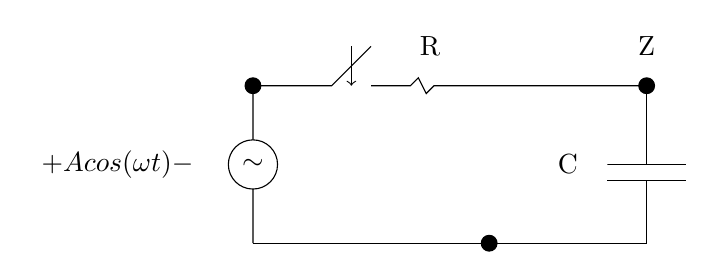
\begin{tikzpicture}
\draw (0,0)--(0,1) node[circle, draw=black,fill=white]{$\sim$}--(0,2)
--(1,2)--(1.5,2.5) (1.5,2)--(2,2)--(2.1,2.1)--(2.2,1.9)--(2.3,2)--(5,2);
\draw (5,2)--(5,1)--(4.5,1)--(5.5,1) (4.5,.8)--(5.5,.8) (5,.8)--(5,0)--(0,0);
\draw [<-] (1.25,2)--(1.25,2.5);
\filldraw (5,2) circle[radius=1 mm];
\filldraw (0,2) circle[radius=1 mm];
\filldraw (3,0) circle[radius=1 mm];
\draw node at (5,2.5) {Z};
\draw node at (2.25,2.5) {R};
\draw node at (4,1) {C};
\draw node at (-1.75,1) {$\begin{matrix}+\\Acos(\omega t)\\-\end{matrix}$};
\end{tikzpicture}
\caption{An RC circuit with AC source. Switch closes when t=0s.}
\label{F:8RC}
\end{center}
\end{figure}

Using nodal analysis for node Z:
\begin{align*}
\frac{Acos(\omega t)-Z}{R}+C\frac{d(0-Z)}{dt}=0\\
RC\frac{dZ}{dt}+Z=Acos(\omega t)
\end{align*}

Using method II, $Z = Z_H+Z_P$. Finding $Z_H$:
\begin{align*}
RC\frac{dZ_H}{dt}+Z&=0\\
Z_H&=Ce^{mt} \rightarrow RCmCe^{mt}+Ce^{mt}=0\\
RCm+1&=0 \rightarrow m=-\frac{1}{RC}\\
Z_H&=Ce^{-\frac{1}{RC}t}
\end{align*}

Next, we determine $Z_P$. Go back to the original equation and make a guess for the form of $Z_P$ that fits the function on the right side of the equation, $Acos(\omega t)$.\par

\begin{align*}
Z_P=k_1cos(\omega t)+k_2sin(\omega t)
\end{align*}

Plugging this in: 
\begin{align*}
RC\frac{dZ}{dt}+Z=Acos(\omega t)\\
-RCk_1\omega sin(\omega t)+RCk_2\omega cos(\omega t)+k_1cos(\omega t)+k_2sin(\omega t)=Acos(\omega t)\\
(-RCk_1\omega+k2) sin(\omega t)+(RCk_2\omega+k_1-A) cos(\omega t)=0
\end{align*}
This can only be true for all times if the coefficients  in front of the sin and cos terms separately equal zero. 

\begin{align*}
-RCk_1\omega+k_2 =0\\
RCk_2\omega+k_1-A=0
\end{align*}

Solve this for $k_1$ and $k_2$ any way you want, but I'll formulate it with matrices.

\begin{align}
\begin{vmatrix}-RC\omega&1\\1&RC\omega \end{vmatrix}
\begin{vmatrix}k_1\\k_2 \end{vmatrix} = \begin{vmatrix}0\\A \end{vmatrix}\\
\begin{vmatrix}k_1\\k_2 \end{vmatrix} = \begin{vmatrix}-RC\omega&1\\1&RC\omega \end{vmatrix}^{-1}
\begin{vmatrix}0\\A \end{vmatrix}\\
\begin{vmatrix}k_1\\k_2 \end{vmatrix} = 
\begin{vmatrix}\frac{A}{R^2C^2\omega^2+1}\\ \frac{ARC\omega}{R^2C^2\omega^2+1} \end{vmatrix}
\end{align}

\begin{clevel}
Show that $\begin{vmatrix}-RC\omega&1\\1&RC\omega \end{vmatrix}^{-1}$ is 
$\frac{1}{R^2C^2\omega^2+1}\begin{vmatrix}-RC\omega&1\\1&RC\omega \end{vmatrix}$. Hint: multiply them and show that you get the identity. What is the inverse of $\begin{vmatrix}-a&1\\1&a \end{vmatrix}$?
\end{clevel}

Returning to our quest of solving for the voltage at node Z:

\begin{align}
Z_P&=\frac{A}{R^2C^2\omega^2+1}cos(\omega t)+\frac{ARC\omega}{R^2C^2\omega^2+1}sin(\omega t) \notag\\
Z&=Z_C+Z_P \notag\\
Z&=Ce^{-\frac{1}{RC}t}+
	\frac{A}{R^2C^2\omega^2+1}cos(\omega t)+\frac{ARC\omega}{R^2C^2\omega^2+1}sin(\omega t)
\label{E:8Z}
\end{align}

Part of this solution will die out as time passes by. This part is called the transient part of the solution. There is another piece of the solution that does not go away with time. This is called the steady state solution.

\begin{alevel}
What are the units of Z?
\end{alevel} 

\begin{alevel}
Which part of this solution would be considered the steady-state solution, $Z_P$ or $Z_C$?
\end{alevel} 

\begin{dlevel}
What constraints on m lead to the homogeneous solution being transient (going away after a long time)?
\end{dlevel}

%%%%%%%%%%%%%%%%%%%%%%%%%%%%%%%%%%%%%%%%%%%%%%%%%%%%%%%%%%%%%%%%%%%%
\section{Frequency Dependance}
You might have noticed that the coefficients $k_1$ and $k_2$ in Equation~\eqref{E:8Z} depend on the angular frequency of the source, $\omega$.\par

For large $\omega$, both $k_1$ and $k_2$ become small. Therefore, the voltage dropped across the capacitor becomes small and most of the voltage is dropped across the resistor. If we think of the circuit from a voltage division perspective, this would make us think the capacitor acts like it has a low \emph{resistance} at high frequencies.\par

\begin{alevel}
What are the units of: $\frac{A}{R^2C^2\omega^2+1}$?
\end{alevel}

\begin{clevel}
Which term goes away faster as the source frequency is increased, the cosine term or the sine term? Come up with an approximate expression for the voltage at node Z at high frequencies and large times. But don't just say, zero. Keep the terms that matter the most.
\end{clevel}


%%%%%%%%%%%%%%%%%%%%%%%%%%%%%%%%%%%%%%%%%%%%%%%%%%%%%%%%%%%%%%%%
\section{Phasor Analysis - Shortcut}
Engineers and scientists need to analyze AC circuits far more complicated than the one shown in Figure~\ref{F:8RC}. Maybe something like this one:

\begin{figure}[H]
\begin{center}
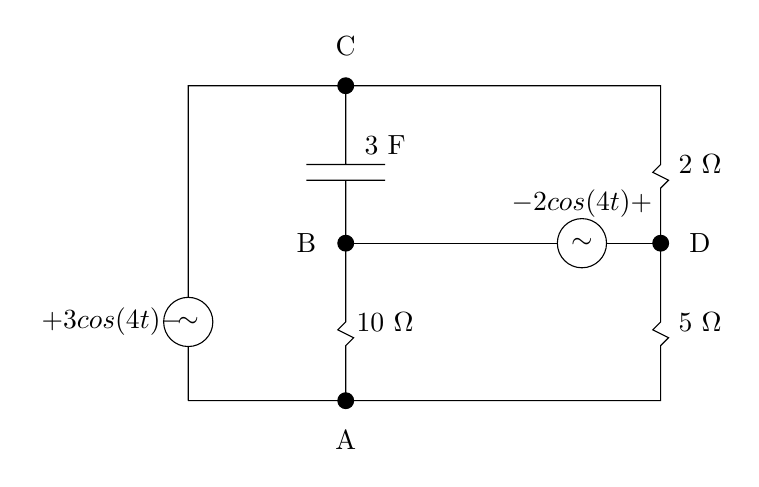
\begin{tikzpicture}
\draw (0,0)--(0,1)node[circle, draw=black, fill=white]{$\sim$}--(0,4)--(2,4)--(2,3)
--(1.5,3)--(2.5,3) (1.5,2.8)--(2.5,2.8) (2,2.8)--(2,2)--(2,1)
--(1.9,.9)--(2.1,.8)--(2,.7)--(2,0)--(0,0);
\draw (2,4)--(6,4)--(6,3)
--(5.9,2.9)--(6.1,2.8)--(6,2.7)--(6,2);
\draw (2,2)--(5,2)node[circle, draw=black, fill=white]{$\sim$}--(6,2);
\draw node at (5,2.5) {$-2cos(4t)+$};
\draw (6,2)--(6,1)
--(5.9,.9)--(6.1,.8)--(6,.7)--(6,0)--(2,0);
\draw node at (-1,1) {$\begin{matrix}+\\3cos(4t)\\-\end{matrix}$};
\draw node at (2.5,1) {10 $\Omega$};
\draw node at (6.5,1) {5 $\Omega$};
\draw node at (2.5,3.25) {3 F};
\draw node at (6.5,3) {2 $\Omega$};
\draw node at (1.5,2) {B};
\draw node at (2,-.5) {A};
\draw node at (2,4.5) {C};
\draw node at (6.5,2) {D};
\filldraw (2,4) circle[radius=1 mm];
\filldraw (2,2) circle[radius=1 mm];
\filldraw (6,2) circle[radius=1 mm];
\filldraw (2,0) circle[radius=1 mm];
\end{tikzpicture}
\caption{AC circuit for analysis}
\end{center}
\end{figure}

If we try to use nodal analysis and brute force math methods, we'll get the right answers, but we'll spend a lot of time crunching trig substitutions and maybe start to dislike engineering (oh no!). In this section, we'll learn a clever technique to speed up the analysis. The key parts to this shortcut are as follows:

\begin{enumerate}
\item To each source, like $V=3cos(4t)$, add to the circuit an imaginary source in series, like $V=i3sin(4t)$. It might seem like we have altered the circuit, and we have. But the real source will produce real currents and voltages and the imaginary source will produce only imaginary currents and voltages. According to superposition the output of interest (perhaps $V_{out}$) will be:

\begin{align}
V_{out}=\underbrace{\rule{2 cm}{.25 mm}}_{real source}+\underbrace{\rule{2 cm}{.25 mm}}_{imag source}
\end{align}

Because we add an imaginary source (and therefore change the circuit), but we must undo that by removing the imaginary part of $V_{out}$ (the part caused by the imaginary source) when we reach the end of the problem.

\item We replace the series combination of the real and complex voltage sources with thier Euler equivalents, like $3cos(4t)+3isin(4t)=3e^{4it}$. See figure~\ref{F:8SI}.

\par
\begin{figure}[H]
\begin{center}
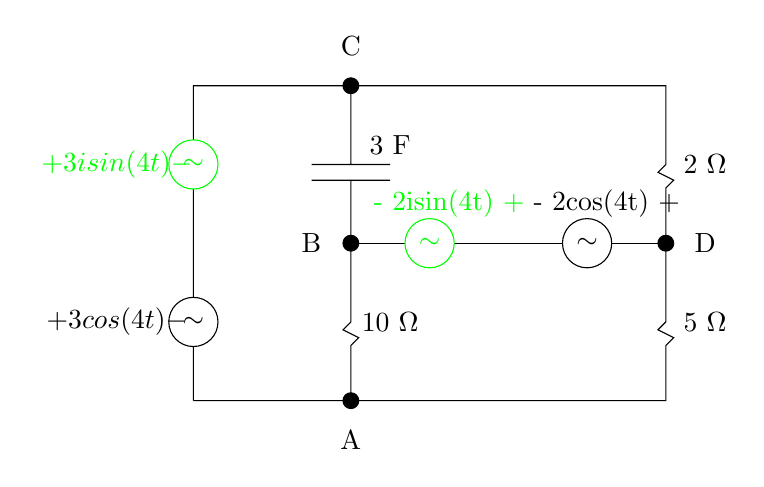
\begin{tikzpicture}
\draw (0,0)--(0,1)node[circle, draw=black, fill=white]{$\sim$}
--(0,3)node[circle, draw=green, text=green, fill=white]{$\sim$}
--(0,4)--(2,4)--(2,3)
--(1.5,3)--(2.5,3) (1.5,2.8)--(2.5,2.8) (2,2.8)--(2,2)--(2,1)
--(1.9,.9)--(2.1,.8)--(2,.7)--(2,0)--(0,0);
\draw (2,4)--(6,4)--(6,3)
--(5.9,2.9)--(6.1,2.8)--(6,2.7)--(6,2);
\draw (2,2)--(3,2)node[circle, draw=green, text=green, fill=white]{$\sim$}
--(5,2)node[circle, draw=black, fill=white]{$\sim$}--(6,2);
\draw node at (5.25,2.5) {- 2cos(4t) +};
\draw node[text=green] at (3.25,2.5) {- 2isin(4t) +};
\draw (6,2)--(6,1)
--(5.9,.9)--(6.1,.8)--(6,.7)--(6,0)--(2,0);
\draw node at (-1,1) {$\begin{matrix}+\\3cos(4t)\\-\end{matrix}$};
\draw node[text=green] at (-1,3) {$\begin{matrix}+\\3isin(4t)\\-\end{matrix}$};
\draw node at (2.5,1) {10 $\Omega$};
\draw node at (6.5,1) {5 $\Omega$};
\draw node at (2.5,3.25) {3 F};
\draw node at (6.5,3) {2 $\Omega$};
\draw node at (1.5,2) {B};
\draw node at (2,-.5) {A};
\draw node at (2,4.5) {C};
\draw node at (6.5,2) {D};
\filldraw (2,4) circle[radius=1 mm];
\filldraw (2,2) circle[radius=1 mm];
\filldraw (6,2) circle[radius=1 mm];
\filldraw (2,0) circle[radius=1 mm];
\end{tikzpicture}
\caption{After adding in two temporary sources}
\label{F:8SI}
\end{center}
\end{figure}


\item We assume all currents and voltages in the circuit ($I_x$,$V_x$) take the form, $I_x=I_{xp}e^{4it}$ and $V_x=V_{xp}e^{4it}$.\footnote{You might agree that all currents and voltages would need to have the same frequency, but couldn't they all have different phases? Yes, they can. The phase angle is clumped in with the constants $I_{xp}$ and $V_{xp}$. Suppose you had kept them seperate, like $I_x=I_{z}e^{4it+\phi}$ then this could be rewritten as $I_x=I_{z}e^{i\phi}e^{4it}=I_{xp}e^{4it}$ where $I_{xp}=I_{z}e^{i\phi}$}
\end{enumerate}

%%%%%%%%%%%%%%%%%%%%%%%%%%%%%%%%%%%%%%%%%%%%%%%%%%%%%%%%%%%%%%%%%%%%%%%%%%%%%%%%
\subsection{Impedance}
Moving forward, we make some observations about the I-V relationships for resistors, capacitors and inductors. Consider the ratio of voltage to current, $\frac{V}{I}$. Let's call this ratio \emph{impedance} and give it a symbol, Z. For a resistor, its impedance would be its resistance\footnote{Ohm's Law}, and would have units of Ohms. 

\begin{alevel}
What are the units of $\frac{V}{I}$ for a resistor? What about for a capacitor? What about the $\frac{V}{I}$ ratio for a Recreator?
\end{alevel}

If we know nothing else about the component in question, we can't do anything else with this expression, $\frac{V}{I}$. However, for AC circuits with sinusoidal inputs, we use the third assumption, that all currents and voltages are of the form, $I_x=I_{xp}e^{4it}$ and $V_x=V_{xp}e^{4it}$. With this assumption, we can determine the impedance of capacitors and inductors.

\begin{align}
\text{Assume: } V=V_pe^{i\omega t}, &I=I_pe^{i\omega t} \notag \\
I=C\frac{dV}{dt}&&V = L\frac{dI}{dt} \notag \\
I = iC\omega V_pe^{i\omega t}&&V = iL\omega I_pe^{i\omega t}\notag \\
I = iC\omega V&&V = iL\omega I \notag \\
\frac{V}{I}=\frac{1}{iC\omega}&&\frac{V}{I}=iL\omega \notag \\
Z_C=\frac{1}{iC\omega}&&Z_L = Li\omega
\end{align}

\begin{clevel}
Fill in the rest of the table.
\end{clevel}

\begin{table}[H]
\begin{tabular}{|c|c|c|c|} \hline
component&Z formula&Z at high freq (high or low)& Z at low freq\\ \hline
resistor&R&R&R \\ \hline
capacitor&$\frac{1}{Ci\omega}$&& \\ \hline
inductor&&&  \\ \hline
\end{tabular}
\end{table}

Because impedance is the ratio of voltage to current, we can use it when implementing loop analysis, nodal analysis and other circuit analysis techniques.\footnote{With AC sources, of course} We treat capacitors and inductors and resistors with the same algebraic relationship and $V=IZ$ and spare ourselves a lot of calculus \footnote{The calculus didn't go away. We just already did it, which is where we got the expressions for impedance in the first place.}.\par

Let's keep going with our example. Replace the sources with their Euler equivalents. Replace the capacitor with a resistor symbol and set its value to its impedance ($\frac{1}{Ci\omega}$).

\par
\begin{figure}[H]
\begin{center}
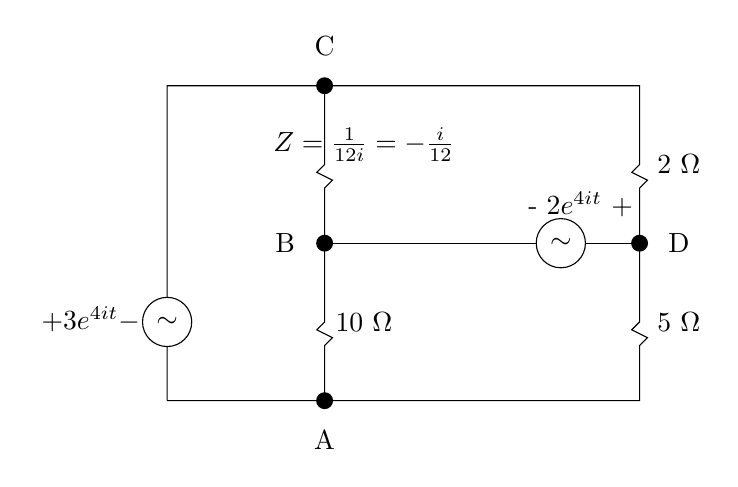
\begin{tikzpicture}
\draw (0,0)--(0,1)node[circle, draw=black, fill=white]{$\sim$}
--(0,4)--(2,4)--(2,3)
--(1.9,2.9)--(2.1,2.8)--(2,2.7)--(2,2)--(2,1)
--(1.9,.9)--(2.1,.8)--(2,.7)--(2,0)--(0,0);
\draw (2,4)--(6,4)--(6,3)
--(5.9,2.9)--(6.1,2.8)--(6,2.7)--(6,2);
\draw (2,2)--(5,2)node[circle, draw=black, fill=white]{$\sim$}--(6,2);
\draw node at (5.25,2.5) {- $2e^{4it}$ +};
\draw (6,2)--(6,1)
--(5.9,.9)--(6.1,.8)--(6,.7)--(6,0)--(2,0);
\draw node at (-1,1) {$\begin{matrix}+\\3e^{4it}\\-\end{matrix}$};
\draw node at (2.5,1) {10 $\Omega$};
\draw node at (6.5,1) {5 $\Omega$};
\draw node at (2.5,3.25) {$Z=\frac{1}{12i}=-\frac{i}{12}$};
\draw node at (6.5,3) {2 $\Omega$};
\draw node at (1.5,2) {B};
\draw node at (2,-.5) {A};
\draw node at (2,4.5) {C};
\draw node at (6.5,2) {D};
\filldraw (2,4) circle[radius=1 mm];
\filldraw (2,2) circle[radius=1 mm];
\filldraw (6,2) circle[radius=1 mm];
\filldraw (2,0) circle[radius=1 mm];
\end{tikzpicture}
\caption{After Euler substition and Impedance Substitution}
\label{F:8SI2}
\end{center}
\end{figure}

Using nodal analysis and writing nodal equations for B and D.

\begin{align*}
\text{Node B: }&\frac{3e^{4it}-B}{-\frac{i}{12}}-I_1+\frac{0-B}{10}=0\\
\text{Node D: }&\frac{3e^{4it}-D}{2}+I_1+\frac{0-D}{5}=0\\
\text{Bonus: }&D=B+2e^{4it}
\end{align*}

Adding the first two equations gives:

\begin{align*}
\frac{3e^{4it}-B}{-\frac{i}{12}}+\frac{3e^{4it}-D}{2}-\frac{B}{10}-\frac{D}{5}=0\\
e^{4it}(36i+\frac{1}{2})-\frac{1}{10}B-(\frac{1}{2}+\frac{1}{5})D=0
\end{align*}

Then substituting the expression for D from the third equation gives:

\begin{align*}
e^{4it}(36i+\frac{1}{2})-\frac{1}{10}B-\frac{7}{10}(B+2e^{4it})=0\\
e^{4it}(36i+\frac{1}{2}-\frac{14}{10})-\frac{8}{10}B=0
\end{align*}

Continuing to solve for B, gives:

\begin{align*}
e^{4it}(36i-0.9)&=\frac{4}{5}B\\
e^{4it}36.01e^{-i88.57^o}&=\frac{4}{5}B\\
B&=1.25*36.01e^{i(4t-88.57^o)}\\
B&=45.01e^{i(4t-88.57^o)}\\
B&=45.01cos(4t-88.57^o)+i45.01sin(4t-88.57^o)
\end{align*}

The second part is imaginary and therefore must be the result of the imaginary sources that were added in. If those sources weren't added in, then the voltage at B would have been: 

\begin{align}
B&=45.01cos(4t-88.57^o)
\end{align}

\begin{alevel}
What would be the impedance of the capacitor if the angular frequency of the source were changed from 4 $\frac{rad}{s}$ to 12 $\frac{rad}{s}$?
\end{alevel}

\begin{alevel}
What would be the impedance of a 2H inductor if the angular frequency of the source were 4 $\frac{rad}{s}$?
\end{alevel}

\begin{blevel}
Rewrite the node equations for the case where the 2 Ohm resistor is replaced with a 2H inductor.
\end{blevel}

\begin{clevel}
Solve for the voltage at B for the case where the 2 Ohm resistor is replaced with a 2H inductor.
\end{clevel}

%%%%%%%%%%%%%%%%%%%%%%%%%%%%%%%%%%%%%%%%%%%%%%%%%%%%%%%%%%%%%%%%%%%
\subsection{Objections}
You might have some objections.\par
\vspace{6pt}
\setlength{\hangindent}{30pt}
\noindent \textbf{Dr. J}
Imaginary numbers don't mean anything. This whole technique is just a mathematical gimmick.\par
\vspace{6pt}
\setlength{\hangindent}{30pt} \noindent \textbf{Cisco}
Imaginary numbers do mean something. They are as real as any other number. There is no such thing as 5. You can have 5 elephants, but not a 5, all by itself.\par
\vspace{6pt}

\setlength{\hangindent}{30pt}\noindent \textbf{Dr. J}
That's exactly my point. You can have 5 elephants but not 5i elephants.\par
\vspace{6pt}

\setlength{\hangindent}{30pt}\noindent \textbf{Cisco}
You can't have $30^0$ elephants either, so does that mean that $30^0$ is a meaningless number? The key for any number is to know what it is trying to represent.\par
\vspace{6pt}

\setlength{\hangindent}{30pt}\noindent \textbf{Dr. J}
So what is 5i trying to represent?\par
\vspace{6pt}

\setlength{\hangindent}{30pt}\noindent \textbf{Cisco}
In the context of circuits?\par
\vspace{6pt}

\setlength{\hangindent}{30pt}\noindent \textbf{Dr. J}
Yes. Let's start with current. What does a complex current mean? Like (5i) Amps?\par
\vspace{6pt}

\setlength{\hangindent}{30pt}\noindent \textbf{Cisco}
The imaginary part encodes two things, one part contributing to the magnitude and one part contributing to the phase. It's similar to a component of a vector - what does the j-hat component mean? Well, it contributes to the magnitude and also to the angle or direction of the vector.\par
\vspace{6pt}

\setlength{\hangindent}{30pt}\noindent \textbf{Dr. J}
What's phase again?\par
\vspace{6pt}

\setlength{\hangindent}{30pt}\noindent \textbf{Cisco}
The phase of a sinusoidal signal indicates how much the peak or a sine or cosine oscillation is shifted in time.\par
\vspace{6pt}

\setlength{\hangindent}{30pt}\noindent \textbf{Dr. J}
So the (5i) Amps means that the current is at an angle? How can a current be at an angle?\par
\vspace{6pt}

\setlength{\hangindent}{30pt}\noindent \textbf{Cisco}
Yes, but its at a phase angle. It would be shifted +90 degrees, which means its graph would be shifted to the left on a I(t) graph.\par
\vspace{6pt}

\setlength{\hangindent}{30pt}\noindent \textbf{Dr. J}
What happens when we multiply that current by a complex resistance, like 2i Ohms?\par
\vspace{6pt}

\setlength{\hangindent}{30pt}\noindent \textbf{Cisco}
Multiplying by i causes a phase shift of 90 degrees. Multiplying by 2 doubles the magnitude. Figure~\ref{F:8COM} shows the number 1, repeated multiplied by i and graphed on the complex plane.\par
\vspace{6pt}

\begin{figure}[H]
\begin{center}
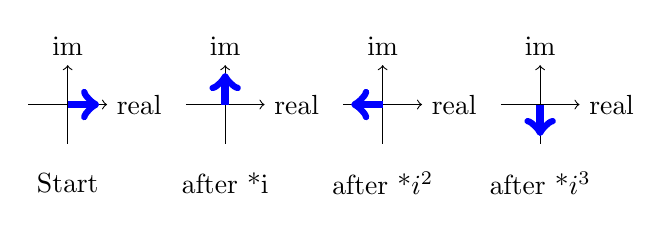
\begin{tikzpicture}
\draw[->] (-.5,0)--(.5,0) node[right] {real};
\draw[->] (0,-.5)--(0,.5) node[above] {im};
\draw [draw=blue, line width=1mm] [->](0,0)--(.4,0);

\draw[->] (1.5,0)--(2.5,0) node[right] {real};
\draw[->] (2,-.5)--(2,.5) node[above] {im};
\draw [draw=blue, line width=1mm] [->](2,0)--(2,.4);

\draw[->] (3.5,0)--(4.5,0) node[right] {real};
\draw[->] (4,-.5)--(4,.5) node[above] {im};
\draw [draw=blue, line width=1mm] [->](4,0)--(3.6,0);

\draw[->] (5.5,0)--(6.5,0) node[right] {real};
\draw[->] (6,-.5)--(6,.5) node[above] {im};
\draw [draw=blue, line width=1mm] [->](6,0)--(6,-.4);

\draw node at (0,-1) {Start};
\draw node at (2,-1) {after *i};
\draw node at (4,-1) {after *$i^2$};
\draw node at (6,-1) {after *$i^3$};
\end{tikzpicture}
\end{center}
\caption{A number being repeatedly multiplied by i.}
\label{F:8COM}
\end{figure}

\setlength{\hangindent}{30pt}\noindent \textbf{Dr. J}
If multiplying by i shifts by $90^0$, does multiplying by i/2 shift by $45^0$?

\setlength{\hangindent}{30pt}\noindent \textbf{Cisco}
Emphatically, no. If you graphed i/2 on the complex plane, it would still be at an angle of $90^0$. If you multiplied something by i/2, the resulting phase would be shifted by $90^0$ but the magnitude would be cut in half. If you wanted to shift something by $45^0$, you would need to multiply by something like (2+2i). This would shift $45^0$ and multiply by $\sqrt{8}$.

\setlength{\hangindent}{30pt}\noindent \textbf{Dr. J}
Suppose we multiply a current of (5i) Amps by impedance (2+2i) Ohms to get some voltage. What does that mean?

\setlength{\hangindent}{30pt}\noindent \textbf{Cisco}
It means that the initial current was phase shifted $90^0$. Then we multiplied by a impedance with a magnitude of $\sqrt{8}$ and a phase shift of $45^0$. This means the impedance will shift the final voltage in phase by another $45^0$ for a total of $135^0$. \footnote{Mathematically, the polar form might illuminate this better, $Z =\sqrt{8}e^{i45^0}$ } The magnitude of the resulting voltage also will be $\sqrt{8}$ times bigger than the current.

\setlength{\hangindent}{30pt}\noindent \textbf{Dr. J}
But it's all just 'math said so.' Math based on math based on more math.

\setlength{\hangindent}{30pt}\noindent \textbf{Cisco}
I don't see it that way. But you might derive Euler's equation a couple times to take away it's magic. 

\setlength{\hangindent}{30pt}\noindent \textbf{Dr. J}
But what about the fact that we had to add in some ficticious sources to make any of this work? Doesn't that make all the intermediate calculations meaningless.

\setlength{\hangindent}{30pt}\noindent \textbf{Cisco}
No. It just means that the intermediate results need interpreting, it does not make them wrong or somehow less related to the physical universe.

%%%%%%%%%%%%%%%%%%%%%%%%%%%%%%%%%%%%%%%%%%%%%%%%%%%%%%%%%%%%%%%%%
\subsection{Example - A motor}
Motors converts electrical energy into motion. Most motors operate on a magnetic principle where an electrical current through a wire causes a magnetic field. This magnetic field might interact with a magnet (or electromagnet) and cause the magnet or the wire to move. 

\begin{clevel}
Suppose a wire were bent into a set of three stacked loops of radius 3 cm. A current of 5A passes through the wire. What is the magnetic field at the center of the hoops? Hint I: Look up how to calculate the magnetic field at the center of a hoop. Hint II: Find the magnetic at the center of one hoop and then add the fields due to each hoop together.
\end{clevel}

Because motors use coils of wire to create significant magnetic fields, they have signficant inductor. Furthermore, the coils might represent a significant length of wire and therefore could have significant resistance. As a result, a motors might be be modeled as an inductor in series with a resistor.\par

Consider the circuit shown in Figure~\ref{F:8MOTOR} where an ac source drives a motor.

\par
\begin{figure}[H]
\begin{center}
\begin{tikzpicture}
\draw (2,0)--(2,1)node[circle, draw=black, fill=white]{$\sim$}--(2,4)--(6,4);
\draw (6,4)--(6,3)--(5.9,2.9)--(6.1,2.8)--(6,2.7)--(6,1);
\draw plot [smooth] coordinates {(6,1) (6.2,.8) (5.8,.6) (5.8,1) (6.2,.6) (6,.5)};
\draw (6,.5)--(6,0);
\draw (6,0)--(2,0);
%\draw (6,2)--(6,1)--(5.9,.9)--(6.1,.8)--(6,.7)--(6,0)--(2,0);
\draw node at (0,1) {$\begin{matrix}+\\170cos(5t) V\\-\end{matrix}$};
\draw node at (7,1) {100 mH};
\draw node at (6.5,3) {2 $\Omega$};
\draw node at (2,-.5) {A};
\draw node at (2,4.5) {C};
\draw node at (6.5,2) {D};
\filldraw (2,4) circle[radius=1 mm];
\filldraw (6,2) circle[radius=1 mm];
\filldraw (2,0) circle[radius=1 mm];
\end{tikzpicture}
\caption{Motor Driven by AC Source}
\label{F:8MOTOR}
\end{center}
\end{figure}

\begin{alevel}
What is the peak source voltage?
\end{alevel}

\begin{blevel}
What is the rms source voltage? What is the frequency of the source, in Hz?
\end{blevel}

Let's try to determine the steady state current through the motor as a function of time. We'll use the same steps as before, but we'll do them faster. 
\begin{enumerate}
\item Add a ficticious source in series with the actual source. ($V=i170sin(5t)$).
\item Replace the two sources with their Euler equivalent, ($170e^{i5t})$
\item Replace the 100mH inductor with the appropriate impedance (0.5i Ohms).\par
\end{enumerate}

The current in this series circuit is then the voltage divided by the total resistance:

\begin{align*}
\text{Approach A}&&\text{Approach B}\\
I = \frac{V_{TOTAL}}{R_{TOTAL}}=\frac{170e^{i5t}}{2+.5i}&&I = \frac{170e^{i5t}}{2+.5i}\\
I=\frac{170e^{i5t}}{2+.5i}\frac{2-.5i}{2-.5i}&&I = \frac{170e^{i5t}}{2.061e^{i14^0}}\\
I=\frac{340-85i}{4.25}e^{i5t}&&I = 82.5e^{-i14^0}e^{i5t}\\
I=(80-20i)e^{i5t}&&\\
I=82.5e^{-i14^0}e^{i5t}&&\\
I&=82.5e^{-i14^0}e^{5it}=82.5e^{5t-14^0}\\
I&=82.5cos(5t-14^0)+i82.5sin(5t-14^0)\\
I&=82.5cos(5t-14^0)
\end{align*}

\begin{alevel}
What is the current when t=1s?
\end{alevel}

\begin{alevel}
Which peak comes first, the peak current through the motor or the peak voltage across the motor?
\end{alevel}

\begin{blevel}
Use the V(I) relationship for an inductor ($V_L=L\frac{dI}{dt}$) to determine the voltage across the inductor as a function of time. What is the rms voltage across the inductor?
\end{blevel}

\begin{blevel}
What is the phase difference between the voltage across the inductor and the current through the inductor? Is this always the case?
\end{blevel}

\begin{blevel}
Use the V(I) relationship for an resistor to determine the voltage across the resistor as a function of time. What is the rms voltage across the resistor?
\end{blevel}

\begin{clevel}
Show that the sum of the $V_R(t)$ plus $V_L(t)$ matches the voltage produced by the ac source.
\end{clevel}

\begin{alevel}
Does the sum of the rms voltages for $V_R$ and $V_L$ equal the rms voltage of the ac source?
\end{alevel}

\begin{clevel}
What value would the inductor need to be for the phase difference between the inductor current and source voltage to be 45 degrees?
\end{clevel}


%%%%%%%%%%%%%%%%%%%%%%%%%%%%%%%%%%%%%%%%%%%%%%%%%%%%%%%%%%%%%%%%%%
\section{RLC AC Circuit. Resonance}
In this section, we'll look at a series RLC circuit with an AC source. 

\par
\begin{figure}[H]
\begin{center}
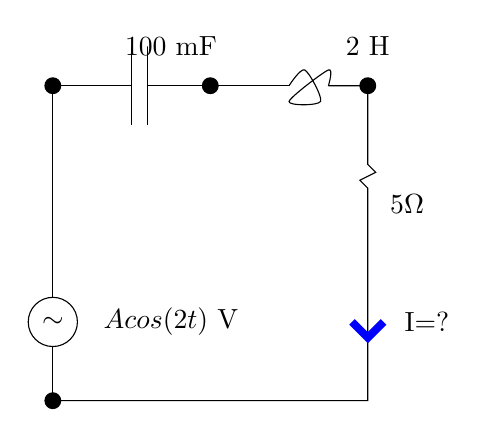
\begin{tikzpicture}
\draw (0,0)--(0,1) node[circle, draw=black, fill=white]{$\sim$}--(0,4)--(1,4);
\draw (1,4)--(1,4.5)--(1,3.5) (1.2,3.5)--(1.2,4.5)--(1.2,4)--(3,4);
\draw plot [smooth] coordinates {(3,4) (3.2,4.2) (3.4,3.8) (3,3.8) (3.5,4.2) (3.5,4)};
\draw (3.5,4)--(4,4)--(4,3)--(4.1,2.9)--(3.9,2.8)--(4,2.7)--(4,0)--(0,0);
\draw [draw=blue, line width=1mm] (3.8,1)--(4,.8)--(4.2,1);
\draw node at (4.75,1) {I=?};
\filldraw (4,4) circle[radius=1 mm];
\filldraw (0,4) circle[radius=1 mm];
\filldraw (0,0) circle[radius=1 mm];
\filldraw (2,4) circle[radius=1 mm];
\draw node at (1.5,1) {$Acos(2 t)$ V};
\draw node at (1.5,4.5) {100 mF};
\draw node at (4.5,2.5) {$5 \Omega$};
\draw node at (4,4.5) {2 H};
\end{tikzpicture}
\caption{Series RLC AC circuit.}
\end{center}
\end{figure}

Let's find the current through the 5 Ohm resistor. First, add in the imaginary sources, replace with Euler equivalent and convert inductance and capacitance to impedence. This time, we'll leave off the $e^{i2t}$ source term until the end.

\par
\begin{figure}[H]
\begin{center}
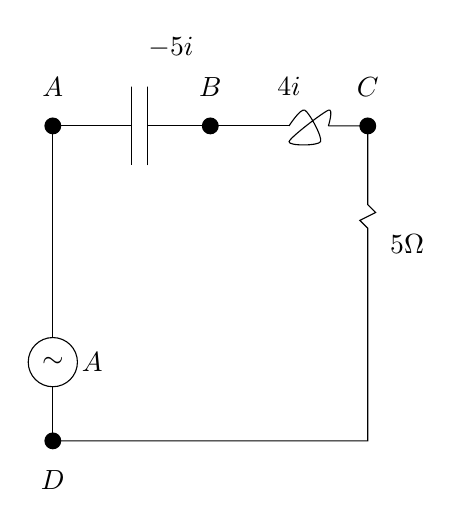
\begin{tikzpicture}
\draw (0,0)--(0,1) node[circle, draw=black, fill=white]{$\sim$}--(0,4)--(1,4);
\draw (1,4)--(1,4.5)--(1,3.5) (1.2,3.5)--(1.2,4.5)--(1.2,4)--(3,4);
\draw plot [smooth] coordinates {(3,4) (3.2,4.2) (3.4,3.8) (3,3.8) (3.5,4.2) (3.5,4)};
\draw (3.5,4)--(4,4)--(4,3)--(4.1,2.9)--(3.9,2.8)--(4,2.7)--(4,0)--(0,0);
\filldraw (4,4) circle[radius=1 mm];\draw node at (4,4.5) {$C$};
\filldraw (0,4) circle[radius=1 mm];\draw node at (0,4.5) {$A$};
\filldraw (0,0) circle[radius=1 mm];\draw node at (0,-.5) {$D$};
\filldraw (2,4) circle[radius=1 mm];\draw node at (2,4.5) {$B$};
\draw node at (.5,1) {$A$};
\draw node at (1.5,5) {$-5i$};
\draw node at (4.5,2.5) {$5 \Omega$};
\draw node at (3,4.5) {$4i$};
\end{tikzpicture}
\caption{AC RLC Circuit.}
\label{F:8R}
\end{center}
\end{figure}

\begin{align*}
I &= \frac{A}{5+4i-5i}\\
I &= \frac{A}{5.1e^{-i11^0}}\\
I &= 0.196Ae^{i11^0} \rightarrow 0.196Ae^{i11^0}e^{2it} && \text{Including the $e^{2it}$ term}\\
I &= 0.196Acos(2t+11^0)
\end{align*}

OK, so the current is phase shifted by 11 degrees and has an amplitude of 0.196A. But you might have noticed something a little interesting - the impedances of the series capacitor and inductor partially cancelled each other out. Both were imaginary, one negative and one positive. Could there be a frequency such that the impedances of the capacitor and inductor are equal and opposite, and cancel out? Yes.

\begin{align*}
\frac{1}{iC\omega}+Li\omega=0 \rightarrow \omega=\frac{1}{\sqrt{LC}}\\
\omega = \sqrt{5} \frac{rad}{s}&&\text{for our numbers}
\end{align*}

If the total impedance from A to C is zero, then the voltage drop from A to C is must also be zero. At this frequency, called the resonance frequency, the current would be easy to recalculate\footnote{Just Ohm's Law - the capacitor and inductor combination has no effect}. $I = 0.2Acos(\sqrt{5}t)$.

\begin{alevel}
Suppose the capacitor were sized to be 0.2 mF. At what angular frequency ($\omega$) will the capacitor and inductor impedances cancel out? Convert this to Hz.
\end{alevel}

\textbf{But wait! Isn't that impossible that the voltage across the inductor and capacitor combination cancels out? There is a changing current passing through the inductor, so the voltage across the inductor can not be zero. One could also argue, successfully, that the voltage across the capacitor also can not be zero.}\par

What gives?\par

Answer: If we calculate the voltages across the capacitor and inductor we will see that, like their impedances, the voltages are indeed not zero, but they are equal and opposite.

\begin{align*}
\text{inductor}			&&\text{capacitor}\\
V_L=2A\frac{dI}{dt}		&&V_C=\frac{1}{0.1}\int_0^t {0.2Acos(\sqrt{5}t)dt}\\
V_L=-0.4A\sqrt{5}sin(\sqrt{5}t)	&&V_C=0.2A\frac{10}{\sqrt{5}}sin(\sqrt{5}t)dt\\
				&&V_C=+0.4A\sqrt{5}sin(\sqrt{5}t)dt
\end{align*}

\begin{clevel}
What is the impedance of a parallel LC circuit at the resonance frequency?
\end{clevel}

\begin{clevel}
Fill in the Table~\ref{T:8R} for the circuit from Figure~\ref{F:8R}.
\end{clevel}

\begin{table}[H]
\begin{center}
\begin{tabular}{|c|c|c|}\hline
component&peak voltage&rms voltage\\ \hline
source&&\\ \hline
resistor&&\\ \hline
inductor&&\\ \hline
capacitor&&\\ \hline
\end{tabular}
\caption{Table summarizing rms and peak values.}
\label{T:8R}
\end{center}
\end{table}

%%%%%%%%%%%%%%%%%%%%%%%%%%%%%%%%%%%%%%%%%%%%%%%%%%%%%%%%%%%%%%%%%%%
\section{An AC Circuit Solved by Four Methods}
In this section, we'll focus on one ac circuit. We'll solve for the current through the 2 $\Omega$ resistor by using the same four techniques we used earlier.\footnote{This problem is designed to help with the technique. This particular circuit is not meant to have any purpose.}

\par
\begin{center}
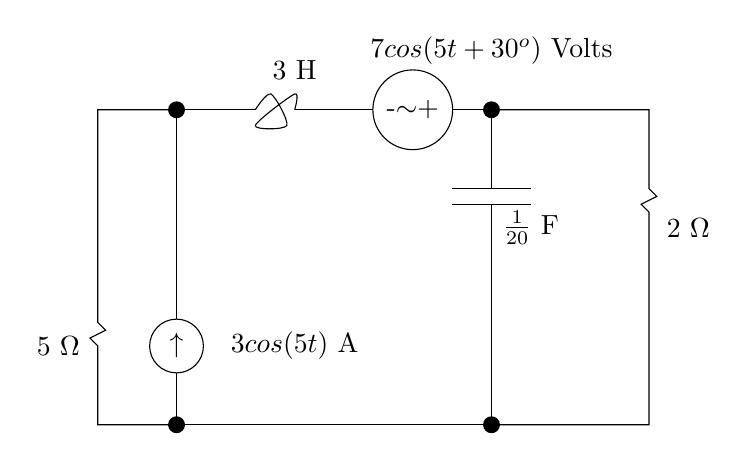
\begin{tikzpicture}
\draw (0,0)--(-1,0)--(-1,1)--(-1.1,1.1)--(-.9,1.2)--(-1,1.3)--(-1,4)--(0,4);
\draw (1,0)--(0,0)--(0,1) node[circle, draw=black, fill=white]{$\uparrow$}--(0,4)--(1,4);
\filldraw (4,4) circle[radius=1 mm];
\filldraw (0,4) circle[radius=1 mm];
\filldraw (0,0) circle[radius=1 mm];
\filldraw (4,0) circle[radius=1 mm];
\draw node at (1.5,1) {$3cos(5t)$ A};
\draw node at (-1.5,1) {5 $\Omega$};
\draw node at (1.5,4.5) {3 H};
\draw node at (6.5,2.5) {2 $\Omega$};
\draw node at (4.5,2.5) {$\frac{1}{20}$ F};
\draw node at (4,4.75) {$7cos(5t+30^o)$ Volts};
%\draw (1,4)--(2,4)--(2.1,4.1)--(2.2,3.9)--(2.3,4)--(3,4);
\draw plot [smooth] coordinates {(1,4) (1.2,4.2) (1.4,3.8) (1,3.8) (1.5,4.2) (1.5,4)};
\draw  (1.5,4)--(4,4);
%--(1.1,2.1)--(.9,2.2)--(1,2.3)--(1,4);
\draw (3,4)node[circle, draw=black,fill=white]{-$\sim$+}--(4,4);
\draw (4,4)--(4,3)--(3.5,3)--(4.5,3) (3.5,2.8)--(4.5,2.8)--(4,2.8)--(4,0)--(1,0);
\draw (4,4)--(6,4)--(6,3)--(6.1,2.9)--(5.9,2.8)--(6,2.7)--(6,0)--(4,0);
\end{tikzpicture}
\end{center}

First, we'll add in the imaginary sinusoidal sources and then use the Euler substitution. Then, we'll replace capacitors and inductors with their impedance values. 

\begin{alevel}
What is the impedance of a $\frac{1}{20}$ F capacitor at a frequency of $\omega=5 \frac{rad}{s}$?
\end{alevel}

The transformed circuit now looks like this:

\par
\begin{figure}[H]
\begin{center}
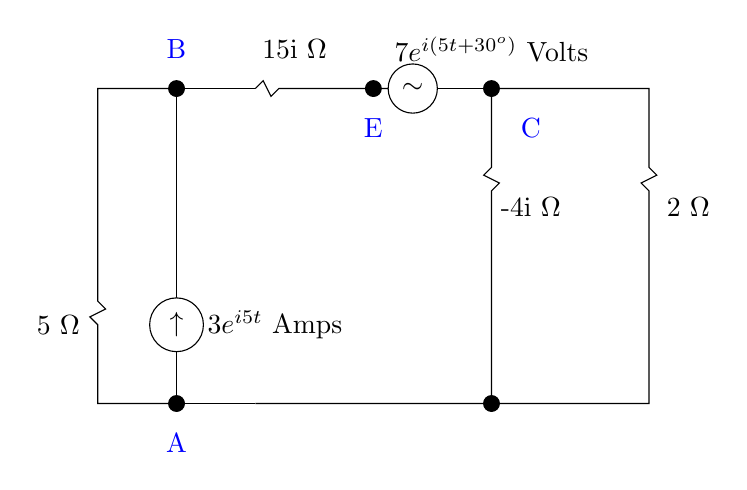
\begin{tikzpicture}
\draw (0,0)--(-1,0)--(-1,1)--(-1.1,1.1)--(-.9,1.2)--(-1,1.3)--(-1,4)--(0,4);
\draw (1,0)--(0,0)--(0,1) node[circle, draw=black, fill=white]{$\uparrow$}--(0,4)--(1,4);
\filldraw (4,4) circle[radius=1 mm];
\filldraw (0,4) circle[radius=1 mm];
\filldraw (0,0) circle[radius=1 mm];
\filldraw (4,0) circle[radius=1 mm];
\draw node at (1.25,1) {$3e^{i5t}$ Amps};
\draw node at (-1.5,1) {5 $\Omega$};
\draw node at (1.5,4.5) {15i $\Omega$};
\draw node at (6.5,2.5) {2 $\Omega$};
\draw node at (4.5,2.5) {-4i $\Omega$};
\draw node at (4,4.5) {$7e^{i(5t+30^o)}$ Volts};
\draw (1,4)--(1,4)--(1.1,4.1)--(1.2,3.9)--(1.3,4)--(2,4)--(3,4);
%\draw plot [smooth] coordinates {(1,4) (1.2,4.2) (1.4,3.8) (1,3.8) (1.5,4.2) (1.5,4)};
%\draw  (1.5,4)--(4,4);
\draw (3,4)node[circle, draw=black,fill=white]{$\sim$}--(4,4);
%\draw (4,4)--(4,3)--(3.5,3)--(4.5,3) (3.5,2.8)--(4.5,2.8)--(4,2.8)--(4,0)--(1,0);
\draw (4,4)--(4,3)--(3.9,2.9)--(4.1,2.8)--(4,2.7)--(4,0)--(1,0);
\draw (4,4)--(6,4)--(6,3)--(6.1,2.9)--(5.9,2.8)--(6,2.7)--(6,0)--(4,0);
\draw node[text=blue] at (0,-.5) {A};
\draw node[text=blue] at (0,4.5) {B};
\draw node[text=blue] at (4.5,3.5) {C};
\draw node[text=blue] at (2.5,3.5) {E};
\filldraw (2.5,4) circle[radius=1 mm];
\end{tikzpicture}
\caption{Circuit after the phasor transformation.}
\end{center}
\end{figure}

%%%%%%%%%%%%%%%%%%%%%%%%%%%%%%%%%%%%%%%%%%%%%%%%%%%%%%%%%%%%%%%%%%%%%%%%%%%%%%
\subsection{Nodal Analysis}
Write out node equations and bonus equations.\footnote{I've left off the $e^{i5t}$ term, like we did for the series RLC AC example. All source terms have it, therefore the solution will have it. We'll just save some writing in the meantime.}

\begin{align}
\text{Node B: }&&\frac{0-B}{5}+3+\frac{E-B}{15i}&=0 \notag\\
\text{Node C: }&&I_1+\frac{0-C}{-4i}+\frac{0-C}{2}&=0\notag\\
\text{Node E: }&&\frac{B-E}{15i}-I_1&=0\notag\\
\text{Bonus 7V Source: }&&C=E+7e^{i30^0}&=E+6.06+3.5i
\end{align}

In matrix form (don't let the complex numbers bother you): 
\begin{align}
\begin{vmatrix}
(-\frac{1}{5}-\frac{1}{15i})	&0	&\frac{1}{15i}	&0\\
0	&(\frac{1}{4i}-\frac{1}{2})	&0	&1\\
\frac{1}{15i}	&0	&(-\frac{1}{15i}) &-1\\
0	&1	&-1	&0
\end{vmatrix}
\begin{vmatrix}
B\\
C\\
E\\
I_1
\end{vmatrix} =
\begin{vmatrix}-3\\0\\0\\6.06+3.5i \end{vmatrix}
\end{align}

Solving using a tool to get the inverse of the matrix and then multiply it by the right side. \footnote{You might try octave online.}

\begin{align}
\begin{vmatrix}B\\C\\E\\I_1 \end{vmatrix} =
\begin{vmatrix} 11.15+5.63i\\0.33-2.42i \\-5.73-5.92i \\.77-1.125i \end{vmatrix}
\end{align}

The current through the 2 Ohm resistor would be the voltage across it (node C) divided by 2 Ohms. Therefore the current is: 

\begin{align*}
I=\frac{0.33-2.42i}{2}=0.167-1.21i=1.22e^{-82.2^0} \text{Amps}\\
\end{align*}

Then tacking back on the $e^{5it}$ and using Euler's relationship:

\begin{align*}
I = 1.22e^{-82.2^0}e^{i5t}=1.22e^{i(5t-82.2^0)}\\
I=1.22cos(5t-82.2^0)+i1.22sin(5t-82.2^0)\\
\end{align*}

Finally, discarding the imaginary part, we get:

\begin{align*}
I=1.22cos(5t-82.2^0) \text{ Amps}
\end{align*}

%%%%%%%%%%%%%%%%%%%%%%%%%%%%%%%%%%%%%%%%%%%%%%%%%%%%%%%%%%%%%%%%%%%
\subsection{Loop Analysis}
Our circuit has three loops and one current source, which has an unknown voltage drop across it (we'll call it $V_x$.) Writing out the loop equations gives:

\begin{align}
\text{Node B: }&&-5I_1-V_x&=0 \notag\\
\text{Node C: }&&V_x-15iI_2+7e^{i30^o}-(-4i)(I_2-I_3)&=0\notag\\
\text{Node E: }&&-(-4i)(I_3-I_2)-2I_3&=0\notag\\
\text{Bonus 3A Source: }&&I_2-I_1&=3
\end{align}

In matrix form:
\begin{align}
\begin{vmatrix}
-5		&0		&0	&-1\\
0		&-15i+4i	&-4i	&1\\
0		&-4i		&4i-2 	&0\\
-1		&1		&0	&0
\end{vmatrix}
\begin{vmatrix}I_1\\I_2\\I_3\\V_x\end{vmatrix} =
\begin{vmatrix}-7e^{i30^o}=0\\-6.06-3.5i\\0\\3\end{vmatrix}
\end{align}

Solving gives:

\begin{align}
\begin{vmatrix}I_1\\I_2\\I_3\\V_x \end{vmatrix} =
\begin{vmatrix} -2.23-1.125i\\0.7696-1.125i \\0.1655-1.208i \\11.15+5.63i \end{vmatrix} \label{E:8M1}
\end{align}

\begin{alevel}
What are the units of the 0.7696 in equation~\ref{E:8M1}? What about the 5.63?
\end{alevel}

We're looking for the current $I_3$, so our answer is:

\begin{align*}
I&=0.1655-1.208i =1.22e^{-82.2^0}\\
I &= 1.22e^{-82.2^0}e^{i5t}=1.22e^{i(5t-82.2^0)}\\
I&=1.22cos(5t-82.2^0)+i1.22sin(5t-82.2^0)\\
I&=1.22cos(5t-82.2^0) &\text{after removing extra source term}
\end{align*}

%%%%%%%%%%%%%%%%%%%%%%%%%%%%%%%%%%%%%%%%%%%%%%%%%%%%%%%%%%%%%%%%%%%%%%%%%%%%%
\subsection{Source Transformations}
We'll solve the same circuit again using source transformations.

\par
\begin{figure}[H]
\begin{center}
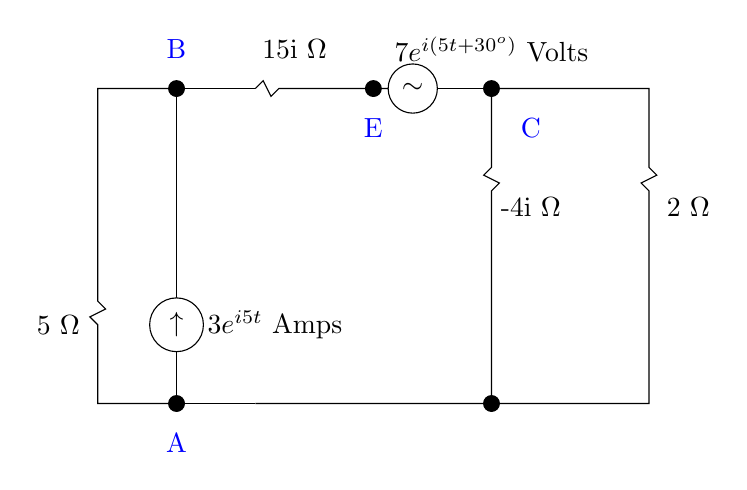
\begin{tikzpicture}
\draw (0,0)--(-1,0)--(-1,1)--(-1.1,1.1)--(-.9,1.2)--(-1,1.3)--(-1,4)--(0,4);
\draw (1,0)--(0,0)--(0,1) node[circle, draw=black, fill=white]{$\uparrow$}--(0,4)--(1,4);
\filldraw (4,4) circle[radius=1 mm];
\filldraw (0,4) circle[radius=1 mm];
\filldraw (0,0) circle[radius=1 mm];
\filldraw (4,0) circle[radius=1 mm];
\draw node at (1.25,1) {$3e^{i5t}$ Amps};
\draw node at (-1.5,1) {5 $\Omega$};
\draw node at (1.5,4.5) {15i $\Omega$};
\draw node at (6.5,2.5) {2 $\Omega$};
\draw node at (4.5,2.5) {-4i $\Omega$};
\draw node at (4,4.5) {$7e^{i(5t+30^o)}$ Volts};
\draw (1,4)--(1,4)--(1.1,4.1)--(1.2,3.9)--(1.3,4)--(2,4)--(3,4);
%\draw plot [smooth] coordinates {(1,4) (1.2,4.2) (1.4,3.8) (1,3.8) (1.5,4.2) (1.5,4)};
%\draw  (1.5,4)--(4,4);
\draw (3,4)node[circle, draw=black,fill=white]{$\sim$}--(4,4);
%\draw (4,4)--(4,3)--(3.5,3)--(4.5,3) (3.5,2.8)--(4.5,2.8)--(4,2.8)--(4,0)--(1,0);
\draw (4,4)--(4,3)--(3.9,2.9)--(4.1,2.8)--(4,2.7)--(4,0)--(1,0);
\draw (4,4)--(6,4)--(6,3)--(6.1,2.9)--(5.9,2.8)--(6,2.7)--(6,0)--(4,0);
\draw node[text=blue] at (0,-.5) {A};
\draw node[text=blue] at (0,4.5) {B};
\draw node[text=blue] at (4.5,3.5) {C};
\draw node[text=blue] at (2.5,3.5) {E};
\filldraw (2.5,4) circle[radius=1 mm];
\end{tikzpicture}
\caption{Circuit redrawn.}
\end{center}
\end{figure}

We'll use these steps.
\begin{enumerate}
\item Combine replace the current source and 5 Ohm resistor with its Thevenin equivalent $(3A,5\Omega)_N \rightarrow (15V,5\Omega)_T$
\item This is in series with the $(7e^{i30^o},15i)_T$. Note that $7e^{i30^o}=6.06+3.5i$. Combining gives $\rightarrow ( (21.06+3.5i) V,(5+15i)\Omega)_T$. The circuit now looks like this:

\par
\begin{figure}[H]
\begin{center}
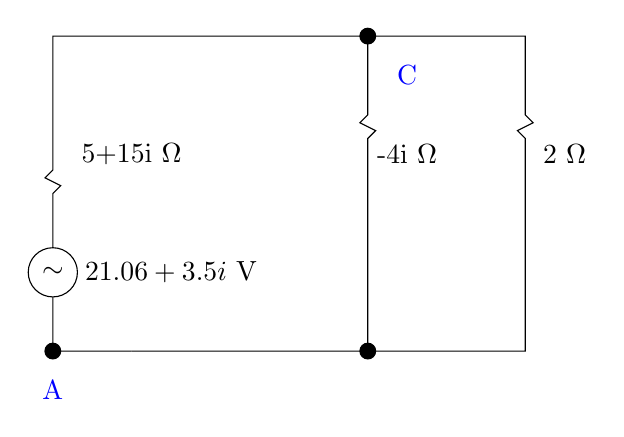
\begin{tikzpicture}
\draw (1,0)--(0,0)--(0,1) node[circle, draw=black, fill=white]{$\sim$}--(0,2)
--(.1,2.1)--(-.1,2.2)--(0,2.3)--(0,4)--(4,4);
\filldraw (4,4) circle[radius=1 mm];
\filldraw (0,0) circle[radius=1 mm];
\filldraw (4,0) circle[radius=1 mm];
\draw node at (1.5,1) {$21.06+3.5i$ V};
\draw node at (6.5,2.5) {2 $\Omega$};
\draw node at (4.5,2.5) {-4i $\Omega$};
\draw node at (1,2.5) {5+15i $\Omega$};
\draw (4,4)--(4,3)--(3.9,2.9)--(4.1,2.8)--(4,2.7)--(4,0)--(1,0);
\draw (4,4)--(6,4)--(6,3)--(6.1,2.9)--(5.9,2.8)--(6,2.7)--(6,0)--(4,0);
\draw node[text=blue] at (0,-.5) {A};
\draw node[text=blue] at (4.5,3.5) {C};
\end{tikzpicture}
\caption{Equivalent circuit, part way through the source transformation process.} 
\end{center}
\end{figure}

\item Transform back to a Norton equivalent $( (21.06+3.5i) V,(5+15i)\Omega)_T \rightarrow (\frac{21.06+3.5i}{5+15i},(5+15i)\Omega)_N$.
 
\item Simplify the current source term. Either multiply top and bottom by complex conjugate (5-15i) or convert to polar form, divide, then convert back to rectangular form. Either way, $\frac{21.06+3.5i}{5+15i} = .631-1.19i$ Amps

\item Combine two parallel impedances, $5+15i$ and $-4i$, to get $\frac{(5+15i)(-4i)}{5+11i}=\frac{60-20i}{5+11i}=0.548-5.21i$. So, total norton equivalent is $( .631-1.194i,0.548-5.21i)_N$

\item Convert back to Thevenin version: 
\begin{align*}
( .63-1.19i,0.548-5.21i)_N& \notag \\
	&\rightarrow ( (.63-1.19i)*(0.548-5.21i),0.548-5.21i)_T \notag \\
	&= (-5.87-3.94i ,0.548-5.21i)_T
\end{align*}
\item Finally, the current through the 2 Ohm resistor is:

\begin{align*}
I&=\frac{-5.87-3.94i}{0.548-5.21i+2}=\frac{-5.85-3.94i}{2.548-5.21i}=0.1655-1.208i &\text{Amps}\\
I &= 1.22e^{-i82.2^0}\\
I &= 1.22e^{-i82.2^0}e^{5it}\\
I &= 1.22cos(5t-82.2^0)+i1.22sin(5t-82.2^0)\\
I &= 1.22cos(5t-82.2^0) &\text{after removing extra source term}
\end{align*}

\end{enumerate}

%%%%%%%%%%%%%%%%%%%%%%%%%%%%%%%%%%%%%%%%%%%%%%%%%%%%%%%%%%%%%%%%%%%%
\subsection{Superposition}
We have two sources, the 3A AC current source and the 7V, phase shifted AC voltage source. Our final current will be:\par

\begin{align}
I=\underbrace{\rule{2 cm}{.25 mm}}_{3 Amp}+\underbrace{\rule{2 cm}{.25 mm}}_{7 Volt}
\end{align}

First, shutting off the 7V source makes that a short circuit. The circuit looks like this:

\begin{figure}[H]
\begin{center}
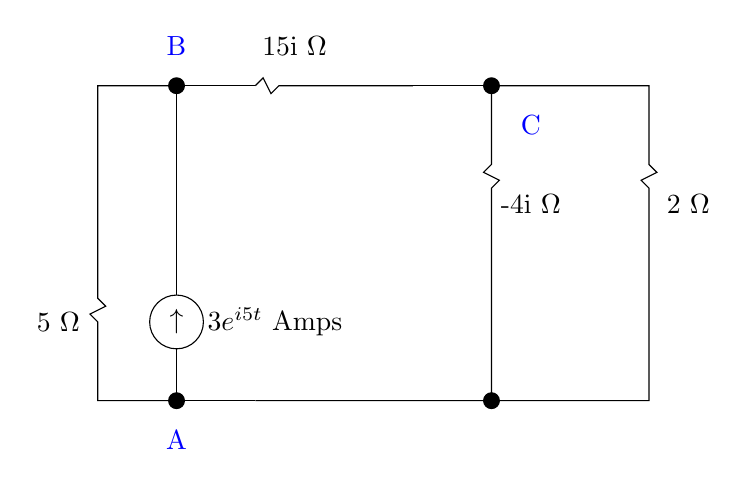
\begin{tikzpicture}
\draw (0,0)--(-1,0)--(-1,1)--(-1.1,1.1)--(-.9,1.2)--(-1,1.3)--(-1,4)--(0,4);
\draw (1,0)--(0,0)--(0,1) node[circle, draw=black, fill=white]{$\uparrow$}--(0,4)--(1,4);
\filldraw (4,4) circle[radius=1 mm];
\filldraw (0,4) circle[radius=1 mm];
\filldraw (0,0) circle[radius=1 mm];
\filldraw (4,0) circle[radius=1 mm];
\draw node at (1.25,1) {$3e^{i5t}$ Amps};
\draw node at (-1.5,1) {5 $\Omega$};
\draw node at (1.5,4.5) {15i $\Omega$};
\draw node at (6.5,2.5) {2 $\Omega$};
\draw node at (4.5,2.5) {-4i $\Omega$};
%\draw node at (4,4.5) {$7e^{i(5t+30^o)}$ Volts};
\draw (1,4)--(1,4)--(1.1,4.1)--(1.2,3.9)--(1.3,4)--(2,4)--(3,4);
%\draw plot [smooth] coordinates {(1,4) (1.2,4.2) (1.4,3.8) (1,3.8) (1.5,4.2) (1.5,4)};
%\draw  (1.5,4)--(4,4);
%\draw (3,4)node[circle, draw=black,fill=white]{$\sim$}--(4,4);
\draw (3,4)--(4,4);
%\draw (4,4)--(4,3)--(3.5,3)--(4.5,3) (3.5,2.8)--(4.5,2.8)--(4,2.8)--(4,0)--(1,0);
\draw (4,4)--(4,3)--(3.9,2.9)--(4.1,2.8)--(4,2.7)--(4,0)--(1,0);
\draw (4,4)--(6,4)--(6,3)--(6.1,2.9)--(5.9,2.8)--(6,2.7)--(6,0)--(4,0);
\draw node[text=blue] at (0,-.5) {A};
\draw node[text=blue] at (0,4.5) {B};
\draw node[text=blue] at (4.5,3.5) {C};
\end{tikzpicture}
\caption{With the 7V source shorted.}
\end{center}
\end{figure}

The voltage from C to A would be, by voltage division:
\begin{align*}
V_C&=\frac{-4i \parallel 2}{-4i \parallel 2 + 15i}V_B \\
V_C&=\frac{-4i \parallel 2}{-4i \parallel 2 + 15i+5}15&& \text{After a source transform}\\
V_C&=\frac{1.6-.8i}{1.6-.8i + 15i+5}15\\
V_C&=\frac{1.6-.8i}{6.6 + 14.2i}15\\
V_C&=-.0489-1.713i\\
I &= \frac{V_C-0}{2}=-0.0245-.856i
\end{align*}

Then, turn the 7V AC source back on and then shut off the 3A AC current source. The circuit looks like this:

\begin{figure}[H]
\begin{center}
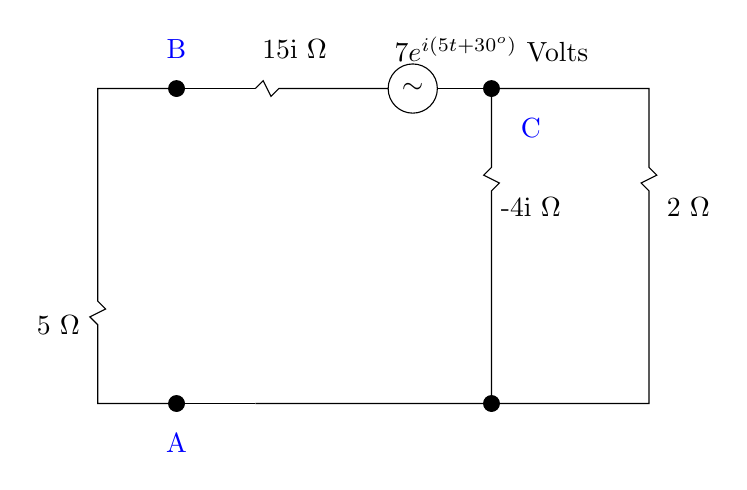
\begin{tikzpicture}
\draw (0,0)--(-1,0)--(-1,1)--(-1.1,1.1)--(-.9,1.2)--(-1,1.3)--(-1,4)--(0,4);
%\draw (1,0)--(0,0)--(0,1) node[circle, draw=black, fill=white]{$\uparrow$}--(0,4)--(1,4);
\draw (0,0)--(1,0) (0,4)--(1,4);
\filldraw (4,4) circle[radius=1 mm];
\filldraw (0,4) circle[radius=1 mm];
\filldraw (0,0) circle[radius=1 mm];
\filldraw (4,0) circle[radius=1 mm];
%\draw node at (1.25,1) {$3e^{i5t}$ Amps};
\draw node at (-1.5,1) {5 $\Omega$};
\draw node at (1.5,4.5) {15i $\Omega$};
\draw node at (6.5,2.5) {2 $\Omega$};
\draw node at (4.5,2.5) {-4i $\Omega$};
\draw node at (4,4.5) {$7e^{i(5t+30^o)}$ Volts};
\draw (1,4)--(1,4)--(1.1,4.1)--(1.2,3.9)--(1.3,4)--(2,4)--(3,4);
%\draw plot [smooth] coordinates {(1,4) (1.2,4.2) (1.4,3.8) (1,3.8) (1.5,4.2) (1.5,4)};
%\draw  (1.5,4)--(4,4);
\draw (3,4)node[circle, draw=black,fill=white]{$\sim$}--(4,4);
%\draw (3,4)--(4,4);
%\draw (4,4)--(4,3)--(3.5,3)--(4.5,3) (3.5,2.8)--(4.5,2.8)--(4,2.8)--(4,0)--(1,0);
\draw (4,4)--(4,3)--(3.9,2.9)--(4.1,2.8)--(4,2.7)--(4,0)--(1,0);
\draw (4,4)--(6,4)--(6,3)--(6.1,2.9)--(5.9,2.8)--(6,2.7)--(6,0)--(4,0);
\draw node[text=blue] at (0,-.5) {A};
\draw node[text=blue] at (0,4.5) {B};
\draw node[text=blue] at (4.5,3.5) {C};
\end{tikzpicture}
\caption{With the 3A source opened up}
\end{center}
\end{figure}

The voltage from C to A would be, by voltage division:
\begin{align}
V_{CA}&=\frac{-4i \parallel 2}{-4i \parallel 2 + 15i+5}7e^{i30^0} \\
V_{CA}&=\frac{1.6-.8i}{1.6-.8i + 15i+5}(6.06+3.5i) \notag\\
V_{CA}&=\frac{1.6-.8i}{6.6+14.2i}(6.06+3.5i)\notag\\
V_{CA}&=(-0.00323-0.114i)(6.06+3.5i)\notag\\
V_{CA}&=.380-.7034i\notag\\
I = \frac{V_{CA}-0}{2}&=0.19-0.352i
\end{align}

Therefore,

\begin{align}
I_{total} &=\underbrace{-0.0245-.856i}_{3 Amp}+\underbrace{0.19-0.352i}_{7 Volt}\\
I_{total} &=0.1655-1.208i\\
I_{total} &=1.22e^{-i82.2^0}\notag\\
I &= 1.22cos(5t-82.2^0)
\end{align}

OK. We made it. The four methods all give the same answer. \par

I must note, that is unlikely that you will go through all of that without some errors. Your answers will not match. Do not give up. Sometimes you might find it helpful to redo a part without looking at your previous work. You might check some calculations with a another student or with a simulation. 

%%%%%%%%%%%%%%%%%%%%%%%%%%%%%%%%%%%%%%%%%%%%%%%%%%%%%%%%%%%%%%%%%%%%%%%%%%%%
\section{Power and AC Circuits}
Power is current times voltage. In an AC circuit, the current and voltage are changing with time and thier peaks might be out of sync with each other. This makes our power calculations a little bit interesting. Read on.\par

%%%%%%%%%%%%%%%%%%%%%%%
\subsection{Example 1. A Resistor}
Consider a 5 Ohm resistor connected to a 10V AC source $V_S=10cos(2t)$. The current would be $I=\frac{V_S}{R}=2cos(2t)$ Amps. The power would be $P=IV=20cos^2(2t) $ Watts. Let's make a couple connections:

\begin{itemize}
\item Because the power is cosine-squared, the power absorbed by the resistor $P=20cos^2(2t)$ must always be positive (or zero).
\item This resembled the case of air drag force acting on a mass on a spring moving through a medium. Positive work is needed to push an object through the medium, regardless of the direction of the force.
\item Max power absorption occurs twice per cycle, once coincident with the positive max voltage and once with the negative max voltage. The frequency of the power formula should therefore be twice the frequency of the applied voltage\footnote{If you use a trig identity on $P=20cos^2(2t)$, you'll see that is the case.}.
\item The average power absorbed in a cycle must be half the max power.  The graph in Figure~\ref{F:8POW} helps to show this\footnote{You could also use a trig identity if you prefer.}.

\begin{figure}[H]
\begin{center}
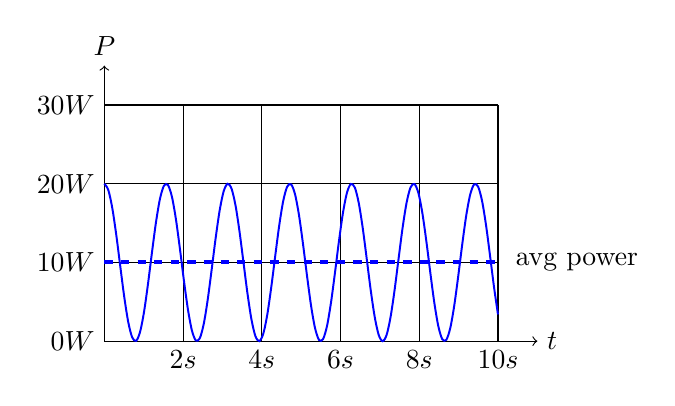
\begin{tikzpicture}
\draw[->] (0,0)--(5.5,0) node[right] {$t$};
\draw[->] (0,0)--(0,3.5) node[above] {$P$};
\draw (0,0)node[left] {$0 W$} (5,0);
\draw (0,1)node[left] {$10 W$} --(5,1);
\draw (0,2)node[left] {$20 W$}--(5,2) ;
\draw (0,3)node[left] {$30 W$}--(5,3) ;
\draw (1,0)node[below] {$2 s$}--(1,3) ;
\draw (2,0)node[below] {$4 s$}--(2,3) ;
\draw (3,0)node[below] {$6 s$}--(3,3) ;
\draw (4,0)node[below] {$8 s$}--(4,3) ;
\draw (5,0)node[below] {$10 s$}--(5,3) ;
\draw [draw=blue, line width=.25 mm,smooth, samples=100,domain=0:10,xscale=.5, yscale=.1] plot(\x,{20*cos(2*57.29*\x)*cos(2*57.29*\x)});
\draw [draw=blue, line width=.5 mm, dashed] (0,1)--(5,1);
\draw node at (6,1) {avg power};
\end{tikzpicture}
\caption{Power absorbed by resistor. The dashed line represents the average power absorbed by the resistor.}
\end{center}
\label{F:8POW}
\end{figure}

\end{itemize}

%%%%%%%%%%%%%%%%%%%%%%%%%55
\subsection{Example 2. A capacitor}
Let's compare this with a capacitor, perhaps a 5 F capacitor connected to a 10V AC source $10cos(2t)$. The current would be $I=5\frac{dV_C}{dt}=-10sin(2t)$. The power would be $P=IV=-100cos(2t)sin(2t)$ Watts. Let's make a couple connections:

\begin{itemize}
\item The power absorbed by the resistor is NOT always positive or negative because the cosine and sine terms are negative at different moments.
\item This is like the spring - it always takes positive work to compress it (spring absorbs positive energy) or to stretch it past its equilibrium position, but then you get the energy back when the spring returns to its equilibrium position (spring absorbing negative energy). Similarly for the capacitor, charges get squished onto the plate of a capacitor twice per cycle, once for negative charges and once for positive charges. The frequency of the power formula should therefore be twice the frequency of the applied voltage.
\item We need to simplify the power formula to see much else. I'll use Euler's relationship:

\begin{align*}
P=-100cos(2t)sin(2t)\\
P = -100(\frac{e^{2it}-e^{-2it}}{2})(\frac{e^{2it}+e^{-2it}}{2})\\
P=-100(\frac{e^{4it}-e^{-4it}}{4})\\
P=-100\frac{cos(4t)}{2}\\
\end{align*}
 
\item From the formula, we can see that positive power absorption occurs at twice the frequency of the applied voltage.  
\item The average power absorbed in a full cycle is zero.\footnote{The average value of a sine or cosine over any number of complete cycles is zero.} Therefore, a capacitor absorbs no net power in an AC circuit.\footnote{For similar reasons, the same is true for an inductor.}
\end{itemize}

\begin{alevel}
What is the power absorbed by a capacitor over two complete cycles?
\end{alevel}

\begin{blevel}
What is the power absorbed by an inductor over two complete cycles?
\end{blevel}

\subsection{General Case}
Many circuits consists of components that are a mix of resistors, capacitors and inductors. Consider some compound component with a current through it of $I=3cos(2t+10^0)$ and a voltage across it of $V=5cos(2t+35^0)$.\\

What is the power absorbed by it as a function of time?

\begin{align}
P=15cos(2t+10^0)*cos(2t+35^0)
\end{align}

This form is difficult to interpret. The max power absorbed is not 15W. Let's try to put this into a form that is easier to interpret by combining the cosines. I'll use an Euler substitution \footnote{You might reasonably use a trig sub here and be done. In this book, I want to reinforce our work with complex numbers and I also see no need to bring in a magic trig sub without proof.}

\begin{align}
P=15cos(2t+10^0)*cos(2t+35^0) \notag\\
P = 15(\frac{e^{i(2t+10^0)}-e^{-i(2t+10^0)}}{2})(\frac{e^{i(2t+35^0)}+e^{-i(2t+35^0)}}{2})\notag\\
P = 15\frac{e^{i(4t+45^0)}-e^{-i(2t+45^0)}+e^{-i25^0}-e^{-i25^0}}{4}\notag\\
P = \frac{15}{2}cos(4t+45^0)+\frac{15}{2}cos(-25^0) \label{E:8POW}
\end{align}

The average value of the first term in Equation~\eqref{E:8POW} for any number of complete cycles is zero. But the second term is just a constant. So the average power dissipation is:

\begin{align}
P_{avg} = \frac{15}{2}cos(-25^0)=\frac{I_{max}V_{max}}{2}cos(-25^0) \notag\\
P_{avg}=\frac{I_{max}V_{max}}{2}cos(25^0)
\end{align}

\begin{alevel}
What is the average value of 5sin(t) between $2\pi$ and $4\pi$ seconds?
\end{alevel}

\begin{blevel}
What is the average power consumption of a component that has a voltage across it of $V=5cos(2t-5^0)$ Volts  and a current through it of $I=5cos(2t+20^0)$ Amps?
\end{blevel}

\begin{clevel}
Consider a component that has a voltage across it of $V=5cos(2t-5^0)$ Volts  and a current through it of $I=5cos(2t+20^0)$ Amps. Assuming we start counting at time 0, how much energy has been absorbed after 2 seconds?
\end{clevel}
